\newpage

\begin{figure}
    \vspace{50pt}
    \centering
    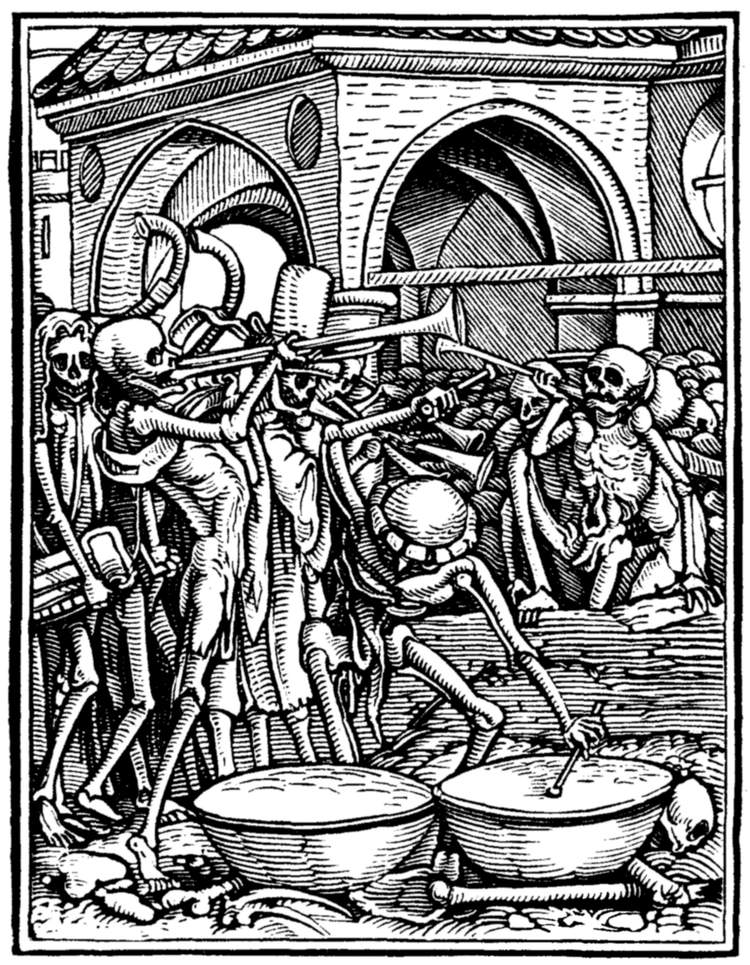
\includegraphics[width=0.5\textwidth]{assets/holbein-ossuary.jpg}
    \\
    \emph{The Ossuary}
    \\
    Hans Holbein
    \\
    \emph{The Dance of Death}
    \\
    (c.1527)
\end{figure}

\begin{center}

\parbox{220pt}{

\eblettrine{T}{his thesis was typeset} using \LaTeX, originally developed by
Leslie Lamport and based on Donald Knuth's \TeX. The body text is set in 11
point Egenolff-Berner Garamond, a revival of Claude Garamont's humanist
typeface, and 10 point Inconsolata. The interactive Python interpreter sessions
and their graphic output were managed by the \emph{abjad-book} tool. Notation
examples were rendered by LilyPond and graph-theoretic examples were rendered
by Graphviz.

}

\end{center}